\documentclass[11pt, letterpaper]{article}
\usepackage[margin=1in,letterpaper]{geometry}
\usepackage{graphicx,float}
\usepackage{hyperref}
\hypersetup{colorlinks = true, urlcolor=blue, filecolor=blue, citecolor = black,linkcolor=black}

\begin{document}
\section{Personal biography}
I, H. M. A. Mohit Chowdhury, started Ph.D. in Computer Science at the University of Colorado at Colorado Springs in Fall 2022. My primary research advisor is Dr. Oluwadare. I will start working as a Graduate Research Assistant with Dr. Boult. I completed my B.Sc. in Computer Science and Engineering in 2017 from Ahsanullah University of Science and Technology, Dhaka. After that, I worked for 5 years as a Software Engineer in national \& multinational companies. At a certain time, I realized that I can contribute by doing research and took decision to pursue Ph.D. degree as a first step. I love site seeing, cooking, bike riding, and gossiping with my friends. My friends call me \textbf{Shadhin} which means \textit{Independent}.

\begin{figure}[H] \center
    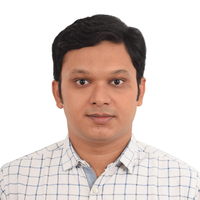
\includegraphics[scale=1]{chowdhury.jpg}
    \caption{H. M. A. Mohit Chowdhury}
    \label{fig:chowdhury}
\end{figure}

\section{One Pixel Attack Git Repository}
Adversarial attack is one of the main concerns in computer vision based algorithms which could demolish a whole system. There are lots of adversarial attacks and one of them is one-pixel attack means changing a single data will cause an unusual result. Here, we can find \href{https://github.com/Hyperparticle/one-pixel-attack-keras}{One Pixel Attack} code for experiencing vulnerability.

\section{Question \& Answer}
\subsection{Question 01}
\subsection{Answer 01}
\subsection{Question 02}
\subsection{Answer 02}
\end{document}